\chapter{Results}
Results would usually encompass benchmarks on the following things:
\begin{itemize}
    \item Time to reconfigure
    \item Time to fault detection
    \item Time to fault mitigation
    \item Fault Mitigation success rate
\end{itemize}
Time constraints and a hardware set-up that is not yet ready to be benchmarked extensively (e.g. benchmarking infrastructure missing, stability problems) only allow us to give us a basic overview over the used resources.

\subsection{Resource Usage}
The design currently uses around 11\% of the Zynqs available hardware resources, a detailed key is given in table \ref{tbl:resourceUtilization}.
Most of the resource usage can be accounted to the \gls{RP} as it contains the Cortex-M1 with its high demand for BRAM elements.
This demand is easily visible in the implemented design (figure \ref{fig:implementation}).
\begin{table}
    \centering
\begin{tabular}{ l | l l l} 
Type    &Used&Available&Percent [\%] used\\
\hline
LUT	    &4827   &53200	&9.07\\
LUTRAM	&289    &17400	&1.66\\
FF	    &4832	&106400	&4.54\\
BRAM    &16	    &140	&    11.42\\
DSP	    &3	    &220	 &   1.36\\
IO	    &25	    &200	 &   12.50\\
BUFG	&3	    &32	    &9.37\\
MMCM	&1	     &4	    &25.00\\
\hline
\end{tabular}
\caption{Resource utilization, post-implemntation}
\end{table}\label{tbl:resourceUtilization}

\begin{figure}[h!]
    \centering
    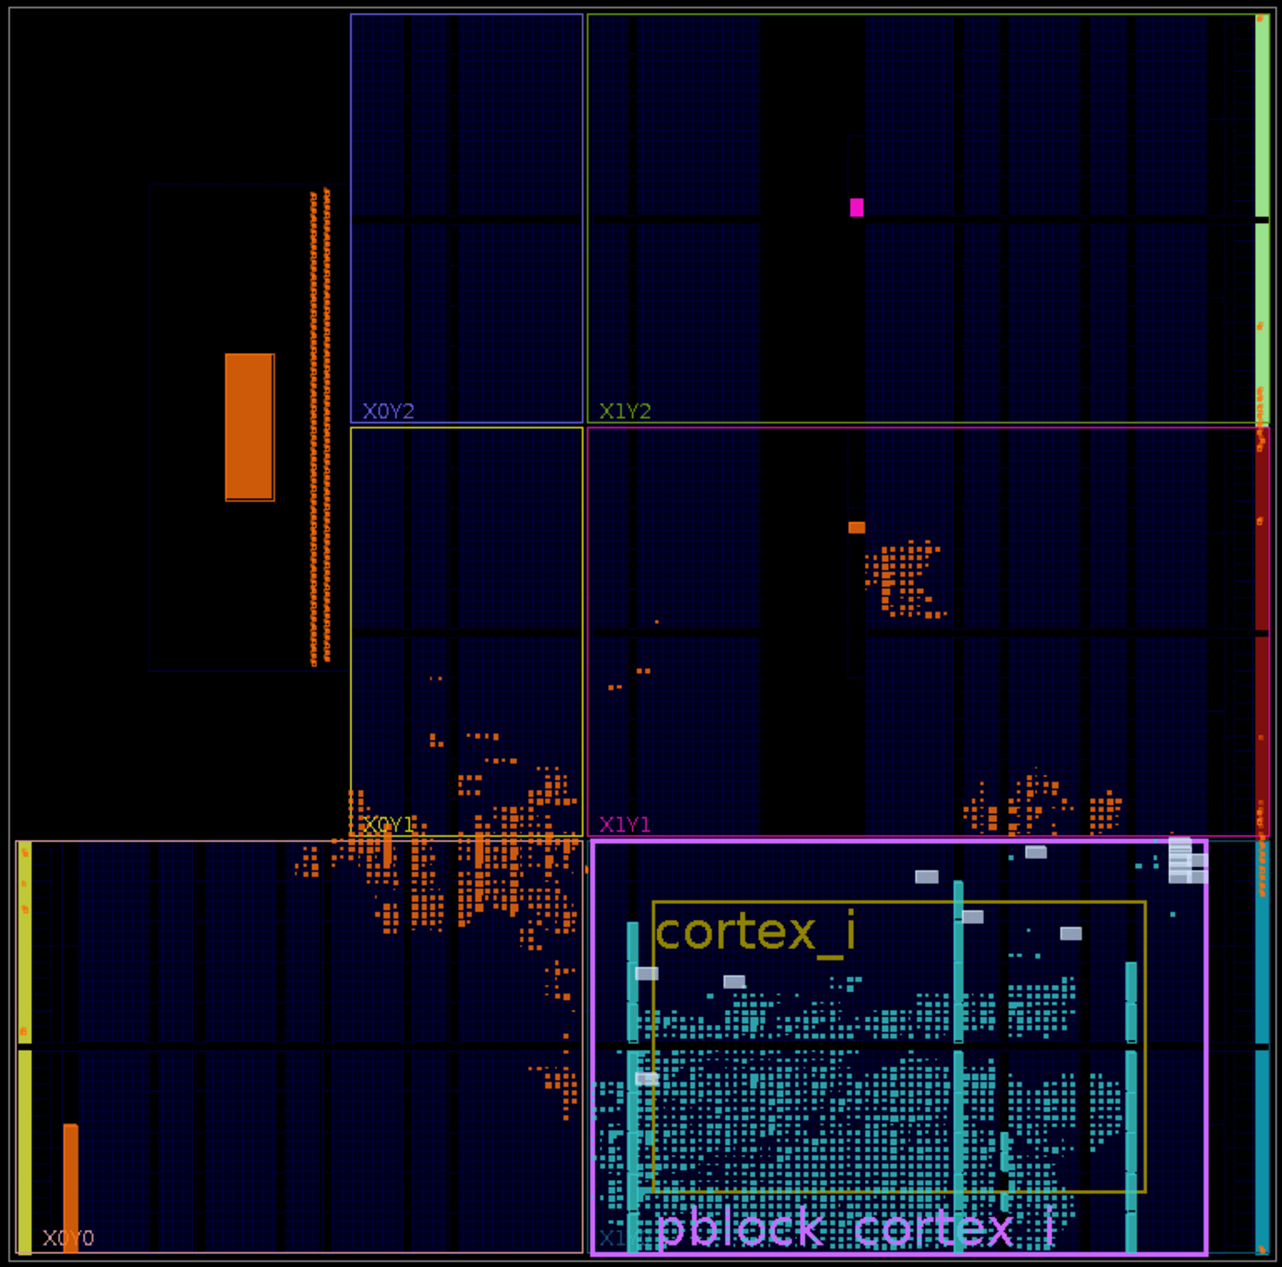
\includegraphics[width=0.75\textwidth]{figures/implementation.pdf}
    \caption{Implemented design, \gls{RP} in the right bottom corner.}\label{fig:implementation}
\end{figure}

\subsection{Open Issues}
\begin{itemize}
    \item Partial reconfiguration fails for one bitstream and results in a voltage drop, see section \ref{sec:voltageDrop}.
    \item Partial Reconfiguration Controller only works with a manual reset after start-up
\end{itemize}
\subsection{Instability of Voltage Supply during \gls{PR}}\label{sec:voltageDrop}
During the process of partial reconfiguration for the Cortex M1 engine module a voltage drop (2V) occurs on the hardware setup.
\begin{figure}[h!]
    \centering
    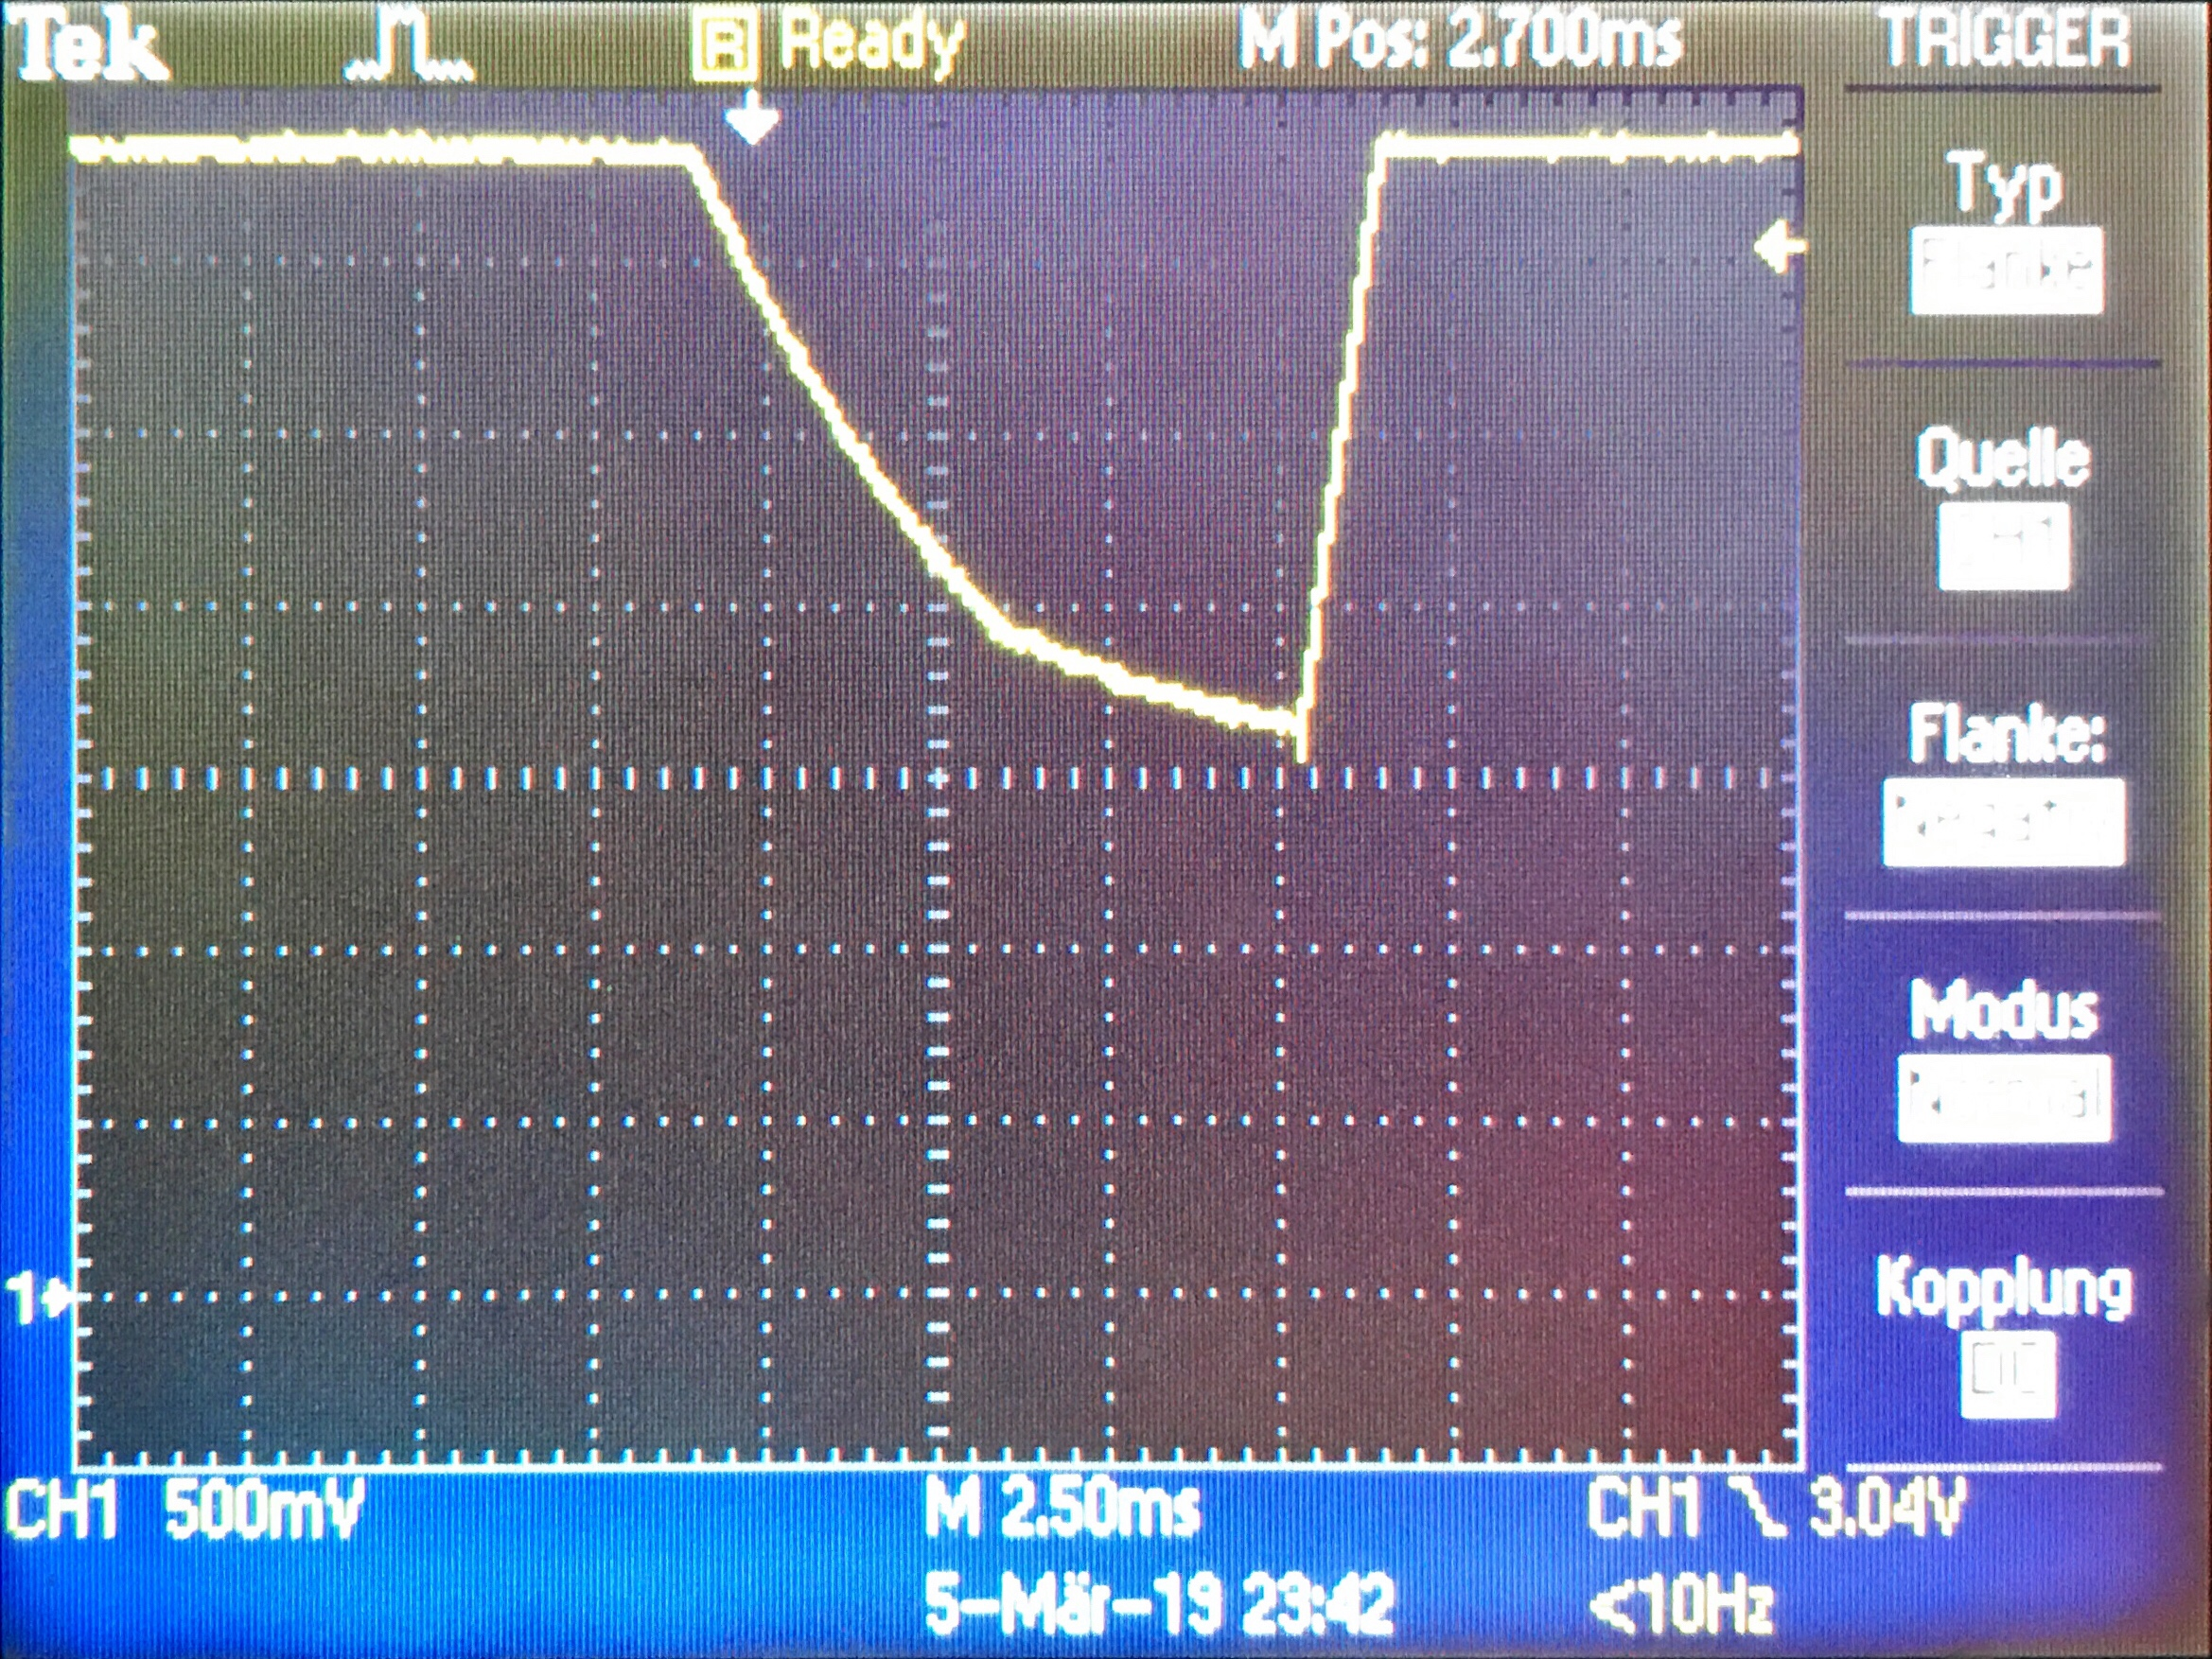
\includegraphics[width=0.75\textwidth]{figures/voltageDropPR.jpg}
    \caption{}\label{fig:voltageDropPR}
\end{figure}
